%!TEX root = ../template.tex
%%%%%%%%%%%%%%%%%%%%%%%%%%%%%%%%%%%%%%%%%%%%%%%%%%%%%%%%%%%%%%%%%%%%
%% chapter2.tex
%% NOVA thesis document file
%%
%% Chapter with the template manual
%%%%%%%%%%%%%%%%%%%%%%%%%%%%%%%%%%%%%%%%%%%%%%%%%%%%%%%%%%%%%%%%%%%%

\typeout{NT FILE chapter2.tex}%

\chapter{Fundamental Concepts}
\label{cha:fundamental_concepts}

This chapter introduces key concepts related to this thesis. Section \ref{sec:digital_heritage_foundation}
provides background of relevant digital aspects in \gls{CH}.
Subsequently, Section \ref{sec:interaction_visualization} explores \glspl{VE}, focusing on user interaction and visualization. 
Section \ref{sec:data} presents diverse \gls{3D} extracting methodologies.
Section \ref{sec:geographic_information_system} examines the role of \glspl{GIS} in applications involving map integration, particularly in the context of archaeological sites. 
The last two sections address important standards, and documentation principles (Section \ref{sub:standart}) to consider when developing heritage applications, as well as a significant European Union initiative (Section \ref{sec:ch_cloud}).
%applications
%concerns
%focused on
%immersive
%covering

\section{Digital Heritage Foundations}
\label{sec:digital_heritage_foundation}

This section covers the fundamental concepts for integrating digital tools to visualize and preserve artefacts during archaeological studies.

\subsection{Digital Cultural Heritage}
\label{sec:digital_heritage}

\gls{CH} includes monuments, sites, landscapes, skills, practices, knowledge and expressions of human creativity~\cite{eu_cultural_heritage}. Collections preserved and managed by public and private bodies - such as museums, libraries and archives - and film heritage are also part of CH. It enriches the lives of people, constitutes a driving force for the cultural and creative sectors, and plays a role in creating and enhancing Europe's social capital.
\gls{CH} can be tangible (castles, museums, works of art), intangible (songs, traditions, etc.), or
digital (born-digital and digitised). In this thesis we will reproduce tangible objects, and represent them in \gls{3D} models digitally.
While policymaking in this area is primarily the responsibility of member states, regional and local authorities, the \gls{EU} is committed to safeguarding and enhancing Europe's \gls{CH}. It does so through a number of policy areas and programmes.


Digital technologies provide new opportunities to preserve cultural content and to make \gls{CH} more accessible to all audiences~\cite{eu_digital_heritage}. Museums and cultural organisations that embrace technology are able to offer innovative visitor experiences, as well as let the public access exhibitions remotely and view material that is not on display.
The \gls{EU} funds an extensive list of projects combining tecnology and art.
Europeana\footnote{\url{https://www.europeana.eu/}} is a European digital platform to empower \gls{CH} in its digital transformation. It supports thousands of European museums, archives and libraries to offer free access to digitalised versions of artworks, books and music.

The visualization of \gls{CH} collections can involve two classes of data: the data constituting the digital cultural object, and
the accompanying metadata, as exemplified below in the Figure \ref{fig:ch_data}~\cite{Windhager2019Visualization}.

\begin{figure}[h!]
    \centering
    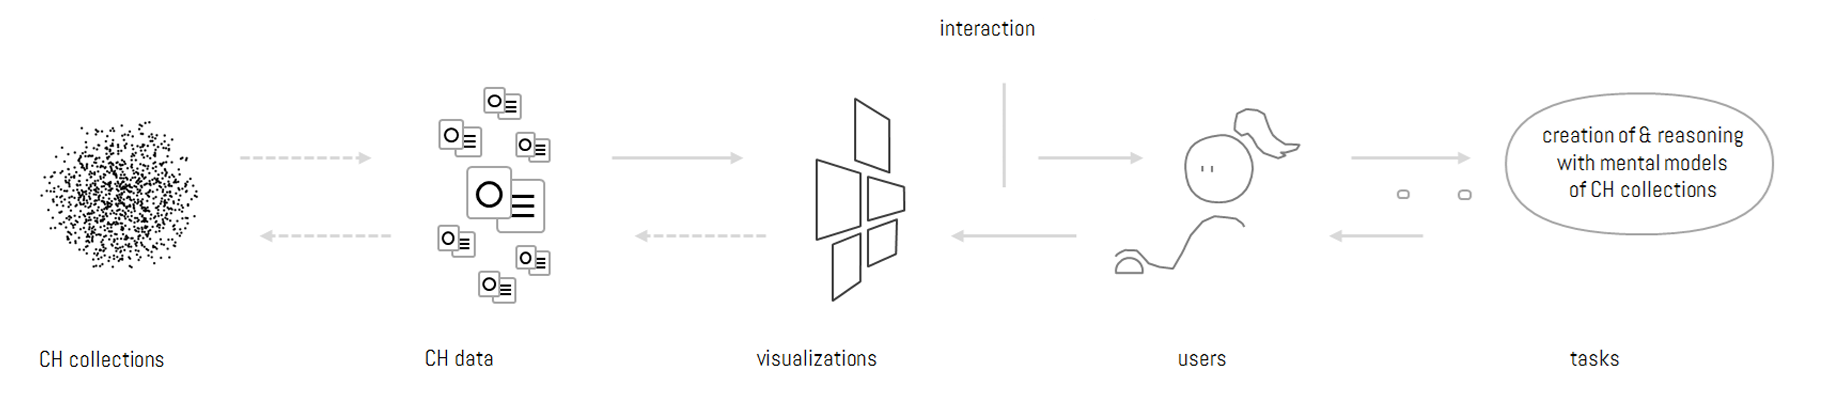
\includegraphics[width=1.0\linewidth]{ch_data}
    \caption{Schematic lineup of a visualization system in the CH data domain~\cite{Windhager2019Visualization}.}
    \label{fig:ch_data}
\end{figure}
\FloatBarrier


The metadata can describe a broad diversity of information associated
with \gls{CH} objects (Figure \ref{fig:ch_objects}), therefore, to systematically classify different types of metadata, it is essential to adopt a unified metadata model. 
Among several standardization initiatives, the \gls{EDM}\footnote{\url{https://pro.europeana.eu/page/edm-documentation}} is one of the most mature efforts. 
The \gls{EDM} reuses several existing Semantic Web vocabularies, such as the metadata set of the \gls{DCMI}\footnote{\url{https://www.dublincore.org/}}, and the
\gls{CIDOC-CRM}\footnote{\url{https://cidoc-crm.org/}} from the \gls{CIDOC} of the International Council of Museums\footnote{\url{https://icom.museum/}}. 
Additionally, the target groups of digital CH collections are very diverse, from museum curators to humanities scholars and from
highly interested enthusiasts to members of the general public— \gls{CH} collections can provide useful and interesting information for all of them. 
%Consequently, many different categorizations of users exist with respect to domain expertise,
%  technical expertise, and motivation of use. There are two significant classes of users, namely experts and casual users. Experts encompass all people with a professional 
% or scientific interest in CH data, whereas casual users are lookin for personally meaningful information in everyday settings.


\begin{figure}[h!]
    \centering
    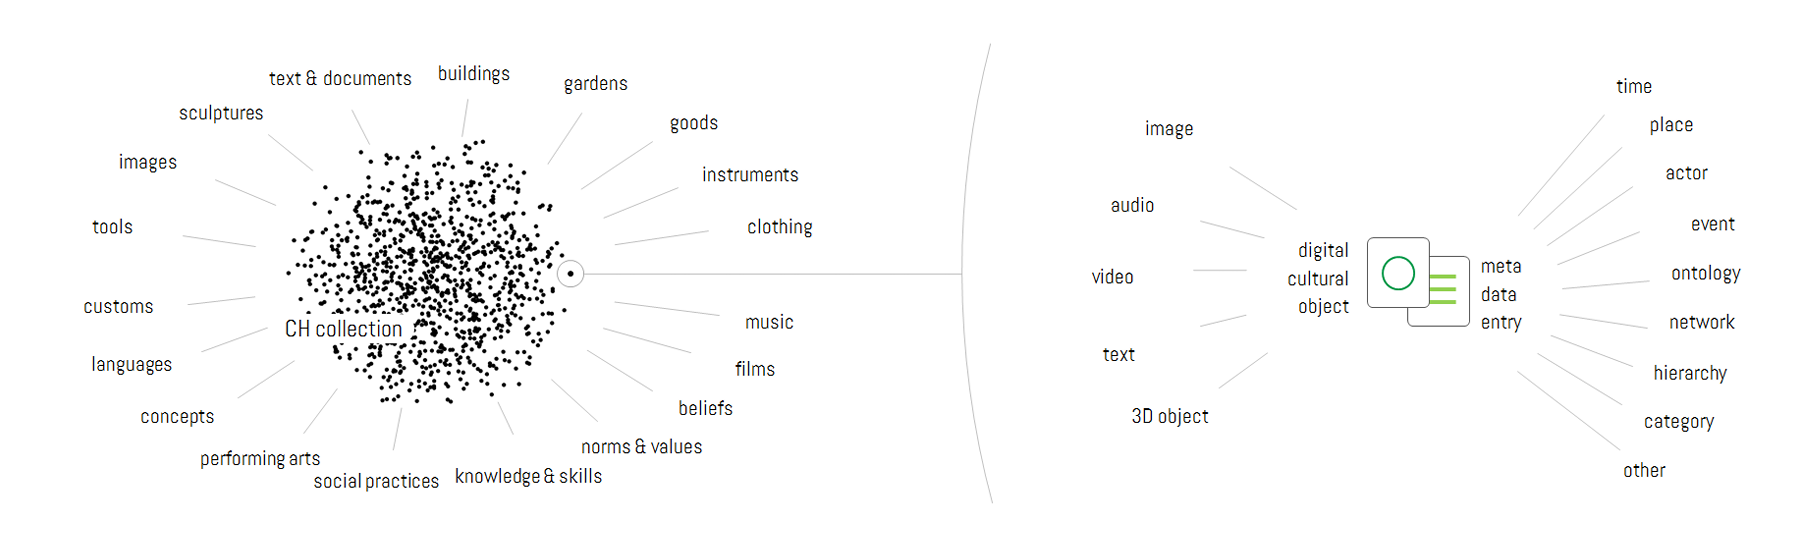
\includegraphics[width=1.0\linewidth]{metadata_entries}
    \caption{Types of cultural objects and related metadata entries~\cite{Windhager2019Visualization}.}
    \label{fig:ch_objects}
\end{figure}
\FloatBarrier


\subsection{Virtual Heritage Environment}
\label{sec:virtual_heritage}

According to Hale and Stanney (2014), "\gls{VE} is a model of reality with which a human can interact, getting information 
from the model by ordinary human senses such as sight, sound, and touch"~\cite{hale2014handbook}. 
It also enables control of the model through typical citizen actions, such as the movement and positioning of body parts and voice. 
Although the terms \gls{VE} and \gls{VR} are frequently used interchangeably, some authors reserve the \gls{VE} for an artificial environment which the user interacts with.

Virtual heritage involves the use of interactive digital technologies to record, preserve, and recreate 
culturally relevant artefacts and sites~\cite{848434}. It allows digitally preserved content to be shared globally, providing an educational experience that enables users to explore \gls{CH} through virtual manipulations of time and space. 
Given the need for interactivity with virtual objects, we naturally will use a \gls{VE} to represent heritage artefacts 
in \gls{3D} in this project, enabling users to explore and interact with \gls{CH} in an immersive and educational way.

Since the 1990s, \gls{VR} was continuously used to recreate historical sites in a virtual immersive environment~\cite{hale2014handbook}. 
This technology provides a way to protect fragile sites while simultaneously educating visitors on how to explore, comprehend, and appreciate significant heritage sites.

\subsection{Digital Twin in Cultural Heritage}
\label{sec:digital_twin}


Generically, the \gls{DT} can be understood as a probabilistic, multiscale,
multiphysics integrated simulation of a system that uses the best physical models,
sensors, and history to mirror the life cycle of its corresponding twin~\cite{dezen2020towards}.
The \gls{DT} consists of three components: physical product in a real monitored
space, data and information connections, and the corresponding virtual product
in virtual space~\cite{grieves2017digital}.


The potential application of the \gls{DT} for heritage is its realistic
representation in the form of an intelligent and semantically enriched \gls{3D} model \gls{HBIM}.
First defined in 2009, HBIM is “a novel solution whereby interactive parametric objects representing architectural elements are constructed from historic data, these elements are accurately mapped onto a point cloud or image-based survey”~\cite{article_hbim}.
This is a powerful tool capable of managing information collected and modeled,
improving its availability and accessibility.
%  According to Nagakura et al. (2015), having a digital model of historical
%  heritage is a cheaper tool to allow building investigations because, unlike other
%  areas of study, there is no way to take buildings to laboratories or store them in
%  museums galleries like other historical artefacts.
Additionally, the use of digital scanning technologies to survey the current state of historic
buildings, such as photogrammetry and laser scanning, expedites the process
of generating a digital model.

% Initially mostly applied in astronautics and aerospace area (Grieves and Vickers,
% 2016), recent progress in IoT (Internet of Things) infrastructures and the development of low-cost
% and reliable sensors has led specialists in building physics to consider such technologies to support
% monitoring strategies for the preservation of heritage sites. 
Implementing \gls{DT} for the management and preservation of \gls{CH} assets requires adopting a collaborative integrated approach and a strong
interplay among heritage recorders, conservation experts and information and communications technology specialists.
In addition to the modelling of information related to heritage sites, open standards should
be adopted for the identification of risks, damage and possible treatments to enable the awareness
of \gls{DT} with respect to their interrelationship and to ensure interoperability among the information
systems of multiple organization and institutions. Before developing preventive conservation strategies, a
good understanding of the heritage site and its context, including the assessment of its multiple values,
is necessary. In this regard, the complex management of information related to the documentation
of heritage places involves critical reflection on the adoption of an appropriate \gls{HIS}. The need for \gls{3D} visualization in \gls{GIS} to enable better
visualization and analysis of complex issues related to elements of significance has led researchers
in the field to progressively consider \gls{HBIM} as a relevant alternative~\cite{jouan2020digital}.


\section{Interaction and Visualization Tecnologies}
\label{sec:interaction_visualization}

This section analyses virtual interactions from a technical perspective, and on the technologies used to create them.
The first subsection (Section \ref{sec:interactors}) lists the various user task interactors. 
Section \ref{sec:hardware_interaction} explores alternative methods of interacting with displays. 
Finally, the last sections discuss how to create a virtual simulation environment and enhance immersive interactions (Section \ref{sec:virtual_reality} and Section  \ref{sec:mix_reality}).

\subsection{Virtual Environment Interactors}
\label{sec:interactors}


A \gls{3D} interactor is generally a geometric object with a defined behavior when certain events 
occur and certain properties of the environment and the objects in it change~\cite{hale2014handbook}.

As is true of \gls{2D} graphical applications, a \gls{3D} environment may contain geometric objects that 
belong to a class that interact with the user and other objects in a well-defined way. In \gls{2D} interfaces, 
these objects are called widgets, components, or interactors and include buttons, menus, scrollbars, 
and pointers. Each class of object encapsulates an interactive behavior, parameterized to allow for 
multiple uses. 



\begin{figure}[h!]
    \centering
    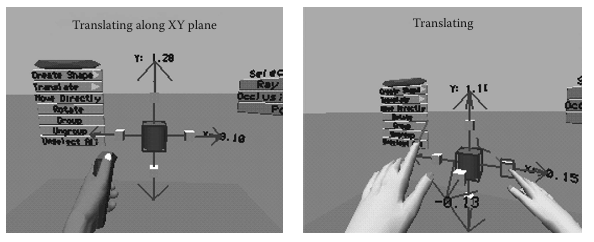
\includegraphics[width=1\linewidth]{human_interaction}
    \caption{\gls{VR} interface where a user is manipulating a \gls{3D} object~\cite{hale2014handbook}.} %Interactors in a shape manipulation task.
    \label{fig:human_interaction}
\end{figure}
\FloatBarrier




Figure \ref{fig:human_interaction} above contains a set of \gls{SVIFT} interactors, including buttons, menus, and tabs
that can be grabbed and moved (or bestow the grab and move ability to another object), constraint maintainers 
(e.g., keeping the manipulated object on a particular plane), and selectors. The image on the left is using a 
ray selector interactor, while the figure on the right is using a poking selector.


\subsection{Hardware Interaction}
\label{sec:hardware_interaction}

This section presents the possible user interactions with \glspl{VE}, achieved through user tasks using input controllers and output devices connected to physical displays.

\subsubsection{Input Devices}
\label{sec:input_devices}

Common \gls{VE} input devices include \gls{6-DOF} trackers\footnote{\url{https://www.ar.rocks/glossary/6dof-tracking}} as exemplified in Figure \ref{fig:input_device}, continuous posture-recognition gloves, discrete 
event gloves, pen-like devices, simple button devices, and special-purpose devices such as the 
Spaceball or force-feedback joysticks. 

In the next paragraphs, I will describe four common available VE task categories.

Selection is the process of specifying an object or set of objects for a particular action. 
Most selection techniques can be categorized based on how an object is indicated, whether
by touching it with a virtual hand, pointing at it, occluding it, encapsulating it within a volume, or 
selecting it indirectly.

Manipulation refers broadly to the  modification of 
attributes of the selected object. Attributes may include position, orientation, scale, shape, color, 
or texture. For the most part, research has mainly considered the manipulation of the  position 
and orientation of rigid objects, although some special-purpose applications include object deformation or scaling. Object manipulation tasks have importance in such applications as design, 
prototyping, simulation, and entertainment, all of which may require environments that can be 
modified by the user. The design space for manipulation techniques is quite large. To provide a simple overview of the 
techniques already developed in the design space, three categories are presented in the following—
virtual hand, proxy, and indirect. 

Travel, also called viewpoint motion control, is the most ubiquitous and common \gls{VE} interaction 
task—simply the movement of the user within the environment. Travel and wayfinding make up the task of navigation. 
Most travel techniques can be categorized as physical locomotion, steering, automated, or manual manipulation. 
Many of the other interactions found in VE applications fall under the heading of system control. 

System Control includes commands, mode changes, and other modifications of system state. 
Often, system control tasks are composites of the other universal tasks. For example, choosing
a menu item is a selection task, whereas dragging an object to a trash can for deletion is a 
manipulation task. The categories of system control techniques include graphical 
menus, voice commands, gestures, and tools.


\begin{figure}[h!]
    \centering
    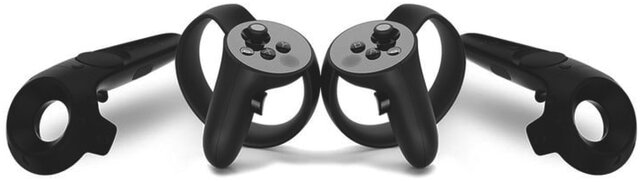
\includegraphics[width=0.60\linewidth]{input_device}
    \caption{HTC Vive controllers(center) and Oculus Touch controllers(at the ends)~\cite{article_input_devices}.}
    \label{fig:input_device}
\end{figure}


\subsubsection{Output Devices}
\label{sec:output_devices}

The three common \gls{VE} display devices are \glspl{HMD}, as illustrated in Figure \ref{fig:HMDs}, \glspl{SID} (fully or 
semisurrounding displays, such as the \gls{CAVE}\footnote{\url{https://steantycip.com/vr-cave/}}) (Figure \ref{fig:HMD1}), and single-screen stereo displays, such as the Responsive Workbench\footnote{\url{https://graphics.stanford.edu/projects/RWB/}}. 
These display types have very different characteristics, and interaction with these displays is likely to be extremely different as well, as shown in Figure \ref{fig:display}. \glspl{HMD} and fully surrounding \glspl{SID} provide the ability to view the entire \gls{VE} by physically turning. Semisurrounding \glspl{SID} require the use of virtual rotations, so applications intended for such 
displays should be designed in a manner to minimize these less-desirable rotations. \glspl{HMD} that have a narrow \gls{FOV} require extensive head rotation in order for the user to see the entire environment. 

%These active stereoscopic glasses are augmented with a constellation of reflective balls that clips onto the frame. The reflective balls work with video tracking that calculates the position of the glasses by triangulating on arrangement of the reflections.

\begin{figure}[h!]
    \centering
    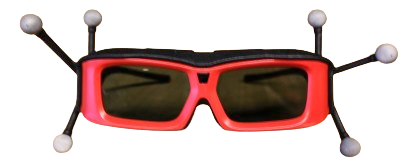
\includegraphics[width=0.5\linewidth]{HMD1}
    \caption{Stereoscopic glasses augmented with a constellation of reflective balls~\cite{SHERMAN2019258}.} 
    \label{fig:HMD1}
\end{figure}

\begin{figure}[h!]
    \centering
    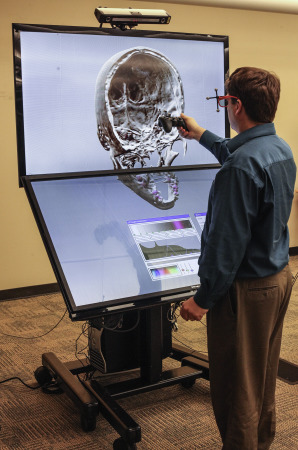
\includegraphics[width=0.25\linewidth]{display}
    \caption{Dual-screen fishtank stereo-capable display~\cite{SHERMAN2019258}.} 
    \label{fig:display}
\end{figure}

\begin{figure}[h!]
    \centering
    \begin{subfigure}[b]{0.3\textwidth}
        \centering
        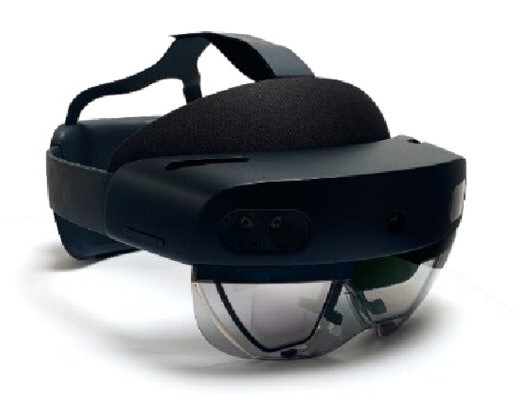
\includegraphics[width=1.0\textwidth]{HMD2}
        \caption{Microsoft HoloLens 2~\cite{headset_article}.}
        \label{fig:HM}
    \end{subfigure}
    \begin{subfigure}[b]{0.3\textwidth}
        \centering
        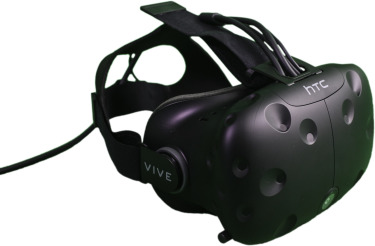
\includegraphics[width=1.0\textwidth]{HMD3}
        \caption{HTC Vive~\cite{SHERMAN2019258}.}
        \label{fig:y1}
    \end{subfigure}
    \hfill
    \begin{subfigure}[b]{0.3\textwidth}
        \centering
        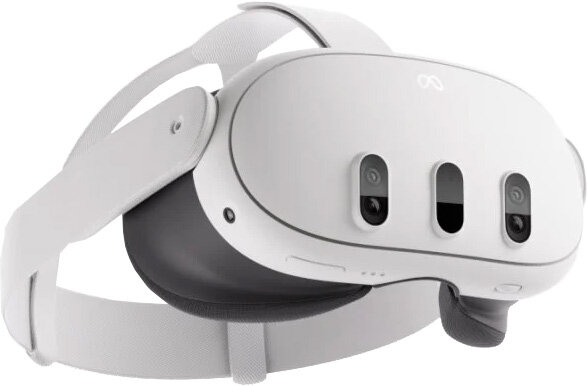
\includegraphics[width=1.0\textwidth]{HMD4}
        \caption{Meta Quest 3~\cite{article}.}
        \label{fig:y2}
    \end{subfigure}
    \caption{Examples of the most recent and advanced \glspl{HMD}.}
    \label{fig:HMDs}
\end{figure}

\FloatBarrier

\subsection{Virtual Reality}
\label{sec:virtual_reality}

\gls{VR} is a sophisticated technology that enables users to engage with a computer-generated environment in an interactive and immersive way. Instead of relying on traditional screens or input commands, \gls{VR} provides users a multisensorial experience. Including move freely, view and navigate in digital spaces from multiple perspectives, and manipulate objects as if they were physically present. This is possible through \gls{VR} devices equipped with motion tracking and controllers, enhancing the sense of presence and realism.

The industry of \gls{VR} combines expertise from diverse disciplines, including engineering, cybernetics, database management, real-time computing, simulation, computer graphics, ergonomics, stereoscopic imaging, anatomy, and even artificial intelligence. Despite its continuously advancements, \gls{VR} still faces significant challenges, such as improving software performance, hardware capabilities, user interaction design, and high-speed network integration.

This project will utilize a \gls{VR} environment which integrates various components to produce an immersive and interactive experience.
This includes the use of digital representations such as \gls{3D} models of glass artefacts and static images of the Troia ruins.
Additionally, the project may incorporate input methods, such as user gestures and touch, allowing for dynamic interactions with the media. 
%By combining these diverse technologies—augmented reality (AR), digital repositories, and real-world artefacts—the project aims to provide a comprehensive platform that enhances the visitor’s experience while preserving and presenting the cultural heritage of Troia.


\subsection{Augmented Reality vs Virtual Reality}
\label{sec:mix_reality}

While \gls{VR} technology, or \gls{VE} as called by Milgram, completely immerses users in a synthetic world
without seeing the real world, \gls{AR} technology augments the sense of reality by superimposing virtual objects and cues upon the real world in real time. 

The Virtuality Continuum is defined by Paul Milgram and Fumio Kishino~\cite{milgram1994taxonomy} as a continuum that spans between the real environment
and the virtual environment comprise \gls{AR} and \gls{AV}
in between, where \gls{AR} is closer to the real world, and \gls{AV} is closer to a pure \gls{VE}, as seen in the Figure \ref{fig:mixed_reality}.

\begin{figure}[htbp]
    \centering
    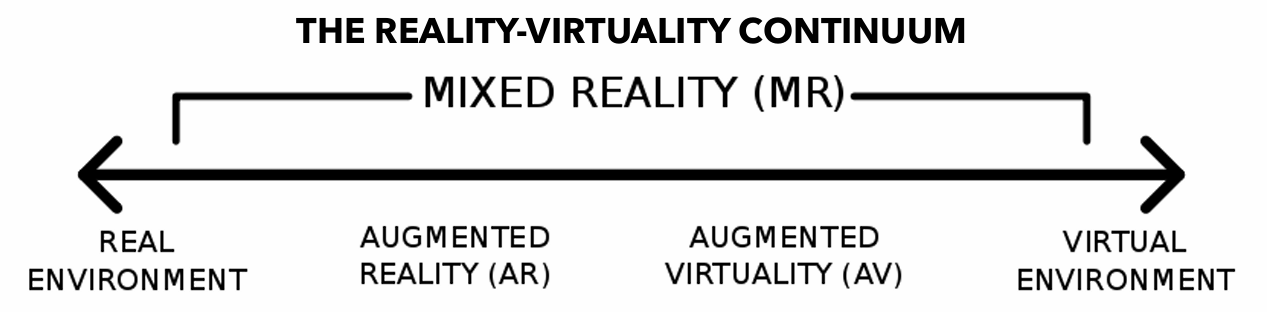
\includegraphics[width=0.8\linewidth]{mixed_reality}
    \caption{Milgram and Kishino’s Virtuality Continuum~\cite{milgram1994taxonomy}.}
    \label{fig:mixed_reality} 
\end{figure} 
\FloatBarrier


\section{\glsentryshort{3D} Data Acquisition and Visualization}
\label{sec:data}

This section describes various techniques used for data acquisition, such as digital cameras and scanners and visualization through 3D models created with advanced software and further enhanced. 
The final subsection explores approaches for artefact reconstruction and the overall process.

\subsection{Photogrammetry}
\label{sec:photogrammetry}

Photogrammetry is a measurement technique that is used to extract the geometry, displacement, and deformation of a
structure using photographs or digital images~\cite{Baqersad2017Photogrammetry}.

Concerning the object(s) of interest and the camera position(s), we distinguish
between terrestrial and aerial photogrammetry~\cite{linder2016digital}.
In aerial photogrammetry, images are acquired via overhead shots from an aircraft, providing topographic maps and land use details. In terrestrial photogrammetry, images are obtained at locations near or on the surface of
the earth and provide detailed dimensional information of an object. When the object size and the camera-to-object 
distance are both less than 100 meters, terrestrial photogrammetry is further defined as close-range photogrammetry. A fundamental technique in photogrammetry for creating accurate \gls{3D} models is Stereoscopic Viewing. 
By capturing two or more images photos of the same object but taken from different positions, it is possible to calculate the \gls{3D} coordinates of any point which is represented in both photos~\cite{linder2016digital}. 
%This method is instrumental in reconstructing object geometries with high precision and is widely applied in topographic mapping, structural analysis, and cultural heritage documentation.  

Multi-image photogrammetry is an advanced technique that combines large groups of images to create detailed \gls{3D} models~\cite{mccarthy2014multi}. The process begins with image acquisition, followed by importing 
the images into specialized software that automatically detects and matches correlated features. This step can be highly time-consuming and demand computer power for large datasets. 
Once matching points are identified, the software calculates their spatial relationships, producing a sparse \gls{3D} point cloud that outlines the subject’s shape, as shown in Figure \ref{fig:photo2}. 
Finally, the software refines this sparse model by reanalyzing the images to generate a much denser point cloud, similar to those produced by laser scanners.
% In photogrammetry the most used model is the central projection.
%It is a geometric procedure that transforms a 3D entity into a 2D reality and it occurs when you have an object, 
%a projection centre and a projection plane oriented in any way with respect to the projected object.
%This projection is then produced because a series of straight lines (or projecting rays) connect the 
%points of the object with the projection centre and, intersecting the projection plane, generate the image points, that are the points projections.
%~\cite{aicardi2018recent}

\begin{figure}[h!]
    \centering
    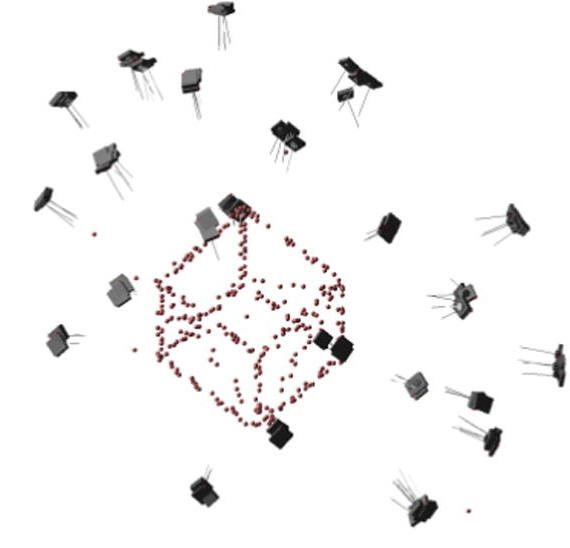
\includegraphics[width=0.45\linewidth]{photogrammetry}
    \caption{131 images of a \gls{3D} object in all-around configuration~\cite{luhmann2016sensor}.}
    \label{fig:photo2}
\end{figure} 
\FloatBarrier

  
The most valuable application of multi-image photogrammetry
may lie in its ability to facilitate community engagement in archaeological documentation.
This approach enables the efficient creation of interactive \gls{3D} models, allowing the public to engage with heritage sites
in a more immersive way than traditional static representations such as site plans and sectional drawings. 
%In the "Previous Work", a close-range photogrammetry technique was used to generate the \gls{3D} excavation model, as detailed in section \ref{sec:photogrammetry_previous}.

\subsection{Light Detection And Ranging (\gls{lidar})}
\label{sec:lidar}

\gls{lidar} sensors enable precise \gls{3D} sensing of objects and are widely used in metrology, environment monitoring, archaeology, and robotics~\cite{li2022progress}.
This technology allows for accurate determination of an object’s distance and velocity. 
Similar to photogrammetry, \gls{lidar} scanning is classified into two main types: terrestrial and airborne.
The three most significant approaches in \gls{lidar} technology are mechanical, nanophotonics-based, and solid-state.
In traditional \gls{lidar} sensors, as shown in Figure \ref{fig:mechanical_LIDAR}, a mechanical rotator is used for optical beam scanning, which introduces limitations on their reliability, size, and cost.

 
\begin{figure}[h!]
    \centering
    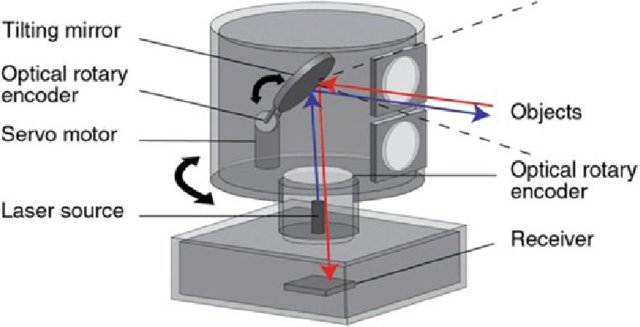
\includegraphics[width=0.6\linewidth]{mechanical_LIDAR}
    \caption{Mechanical Spinning \gls{lidar}~\cite{inbook}.}
    \label{fig:mechanical_LIDAR}
\end{figure} 
\FloatBarrier


Solid-state \gls{lidar} presents an alternative to traditional \gls{lidar} by eliminating the need for a bulky mechanical rotator. %, visualization example in Figure \ref{fig:flash_based}.
Moreover, advancements in optical technology have led to the development of nanophotonics-based devices with high potential and superior advantages for \gls{lidar} sensors. %An example of its usage in Figure \ref{fig:sequential_ilumination}. 
Different scanning techniques produce diverse types of scan outputs. For instance, flash-based \gls{lidar} from solid-state approach captures a full-frame \gls{3D} image in a single snapshot, as shown in Figure \ref{fig:flash_based}, while sequential illumination-based \gls{lidar} scans objects by sequentially illuminating small regions, producing the whole frame, as depicted in Figure \ref{fig:sequential_ilumination}. \\

\begin{figure}[h!]
    \centering
    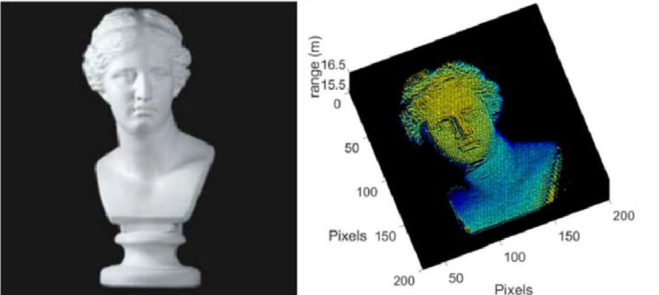
\includegraphics[width=0.65\linewidth]{flash_based}
    \caption{Flash-based \gls{lidar} sensor. \small{Left: \gls{2D} image of sensing target, Right: Captured \gls{3D} image}~\cite{li2022progress}.}
    \label{fig:flash_based}
\end{figure} 

\begin{figure}[h!]
    \centering
    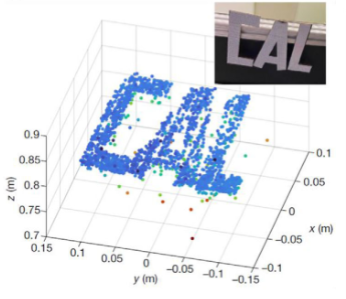
\includegraphics[width=0.45\linewidth]{sequential_ilumination}
    \caption{A \gls{lidar} sensor based on sequential illumination~\cite{li2022progress}.}
    \label{fig:sequential_ilumination}
\end{figure} 

\FloatBarrier

\subsection{Artifacts Reconstruction}
\label{sec:reconstruction}

Systems capable of automatically reconstructing objects from their fragments can greatly aid in the study of many civilizations~\cite{willis2008computational}.
Automated reconstruction systems working from large databases of digitized fragments could uncover numerous partial or
complete reconstructions of artefacts that may have been excavated during different years of the same excavation, or possibly
from different sites altogether. In this way, reconstruction systems not only save researchers time but, given a sufficient database 
of fragments, also have the capacity to reconstruct artefacts that would have otherwise remained as an incoherent pile of disjoint fragments~.

Precise shape measurement can be achieved using advanced laser scanners or other commercially available shape measuring devices based on stereo 
vision or structured light~\cite{7801178}. A detailed triangulated \gls{3D} model of a corrupted shape is the prerequisite for its subsequent reconstruction. 
Missing or scarred parts of a shape can be reconstructed from similar parts either from the same
object or by using a similar object as reference. If an object has symmetrical features, the missing or damaged part can be restored by copying the undamaged side.
To fix scar parts or gaps, a mathematical technique called surface spline patches is used to smoothly fill in and blend the missing areas.

\section{Geospatial Data and Systems}
\label{sec:geographic_information_system}

A \acrfull{GIS} is a computer system for capturing, storing, checking, and displaying data related to positions on Earth’s 
surface~\cite{natgeo_2024}. By relating seemingly unrelated data integrated by geographical location, \glspl{GIS} can help individuals and organizations understand spatial patterns and relationships.

In the context of \gls{GIS} and geospatial data, two of the most prominent community initiatives are the \gls{OGC}\footnote{\url{https://www.ogc.org/}} and the \gls{OSGeo}\footnote{\url{https://www.osgeo.org/}}.  
The \gls{OGC} is an international voluntary consensus standards organization, constituting more than 450 strong united organizations (such as Esri\footnote{\url{https://www.esri.com/}}, Nasa\footnote{\url{https://www.nasa.gov/}}). The consortium publishes open standards that ensure interoperability between diverse \gls{GIS}\footnote{\url{https://ogcapi.ogc.org/}}.
The \gls{OSGeo} is an organization that promotes global adoption of open geospatial technology through an open philosophy and community driven development. 
For this project, the standards established by the \gls{OGC} and the open resources provided by \gls{OSGeo} are particularly relevant. 
These resources enable the creation of data from public geographic databases, supporting the development of interactive maps and ensuring the interoperability of geospatial data.

The first subsection provides an overview of geospatial data and its usage, while the following section explores its applications in archaeology.

\subsection{Geospatial Data} 
\label{sub:geospatial_data}

\gls{GIS} applications may include diverse spatial data types, such as cartographic data, photo-
graphic data, digital data, or data in spreadsheets. Once all the desired data have been
entered into a \gls{GIS} system, they can be combined to produce a wide variety of maps,
that highlight different spatial relationships depending on the selected data layers. 
One of the most common uses of
\gls{GIS} technology involves comparing natural features with human activity, as illustrated in Figure \ref{fig:gis}.

Maps help visualize relationships between spaces and objects in proximity, aiding spatial analysis to identify patterns and make informed decisions based on data.
A classic example of this geographic method is Jon Snow's study during the cholera epidemic in London in 1854~\cite{inbook}. Jon Snow plotted the locations of cholera cases against the location of water pumps and noticed that the epidemic was concentrated in a certain neighborhood. 
Through the causal linkages, it was proven that when the contaminated pump was closed, the epidemic quickly came to a halt. 
A map of just the water pumps or incidences of cholera would have been of little value, but combining both revealed the contaminated source. 

\begin{figure}[h!]
    \centering
    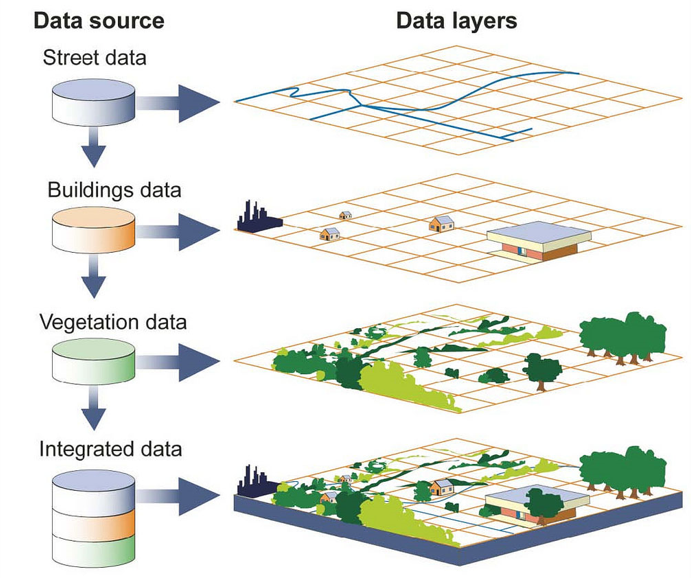
\includegraphics[width=0.50\linewidth]{gis}
    \caption{Visual Representation of Data Layers Integration in a \gls{GIS}~\cite{gao_data_layers}.}
    \label{fig:gis}
\end{figure}

\subsection{GIS Applications in Archaeology}
\label{sub:gis_archeology}

The application of \gls{GIS} in archaeology has brought about a transformative shift, equipping archaeologists with powerful tools to collect, analyze, 
and visualize geospatial data from archaeological sites~\cite{yao2023overview}. Since 2000, archaeologists began employing \gls{GIS} for more complex spatial analyses, including landscape analysis and site distribution 
patterns. Additionally, the development of \gls{3D} \gls{GIS} technology enabled archaeologists to reconstruct ancient sites in virtual environments, offering a 
better understanding and visualization of archaeological site structures and layouts.

A key technology that complements \gls{GIS} in archaeology is \gls{lidar}. 
The employment of \gls{lidar} has been successful as an archaeological surveying tool for locating and identifying
sites, sometimes in very remote and difficult to access locations~\cite{article_lidar}. For example, the recent, and highly publicized, 
discovery of what is believed to be the Mayan site of Ciudad Blanca in Honduras~\cite{Tolley2012}.

\gls{GIS} also serves as an invaluable platform for the comprehensive management of \gls{CH} resources. It excels in handling a wide array of
unstructured data related to \gls{CH}, allowing for a more organized and efficient approach to preservation efforts. One significant 
application of \gls{GIS} is the inventorying of \gls{CH} sites, including archaeological, architectural, and historical locations. Traditional recording methods often face limitations in terms of speed and accuracy when
it comes to gathering and assessing current situation data.

With advancements in \gls{3D} graphics, high-resolution rendering, artificial intelligence, and \gls{3D} printing, those methodologies have progressively found widespread application in the preventive protection and restoration of cultural artefacts. 
In archaeology, \gls{GIS} is essential for managing spatial data, often integrating spatial databases, such as PostgreSQL\footnote{\url{https://www.postgresql.org/}}/PostGIS\footnote{\url{https://postgis.net/}} or Oracle Spatial\footnote{\url{https://www.oracle.com/database/spatial-database}} for efficient data storage and querying.
Moreover, software such as ArcGIS Pro\footnote{\url{https://www.esri-portugal.pt/pt-pt/arcgis/produtos/arcgis-pro}} or QGIS\footnote{\url{https://qgis.org/}} is used to visualize, analyze, and interpret this data. These \glspl{GIS} process archaeological data following specific data standards and protocols.

\section{Heritage Metadata Standards and Documentation} 
\label{sub:standart}

Standards are critical for systematic and robust development of any emerging technology~\cite{hale2014handbook}.
Specification standards provide for practical descriptions of product characteristics and limitations, 
critical to an end user. Interface standards allow for interchangeability of components developed by 
different manufacturers, thus enabling specialization and robust competition in the marketplace. 
Safety standards ensure the health and safety of product users. Finally, terminology standards ensure that 
technical terminology is used in a consistent and rigorous manner, thus preventing confusion and 
ambiguity in scientific and technical reports and specifications.

International standards and ontologies for data encoding are crucial
to speed up interoperability and the process of integration~\cite{eide2008encoding}. \gls{CIDOC-CRM}, which is created to capture the richness typical of CH
information, fully fits our needs: its classes and properties
work perfectly to capture the concepts underlying database structures, providing a high level of data integration.

In the subsections below, the first presents a commonly used model with aggregated standards, followed by a significant European organization in \gls{CH} preservation.

\subsection{\glsentryshort{CIDOC} Conceptual Reference Model} 
\label{sec:cidoc}


The \gls{CIDOC-CRM}\footnote{\url{https://cidoc-crm.org/}} is a theoretical and practical tool for integrating \gls{CH} information~\cite{eide2008encoding}. It provides formal definitions and a structured framework to describe concepts and relationships that support the organization and connection of information regarding \gls{CH} objects and their contexts (Figure \ref{fig:cidoc}).
Since 2006, \gls{CIDOC-CRM} has been recognized as an official ISO standard (\texttt{ISO 21127:2023}). The most recent version establishes \gls{CIDOC-CRM} as a compatible interface for \gls{OGC} standards, enhancing its application in \gls{GIS} and facilitating geospatial and spatiotemporal reasoning.


\begin{figure}[h!]
    \centering
    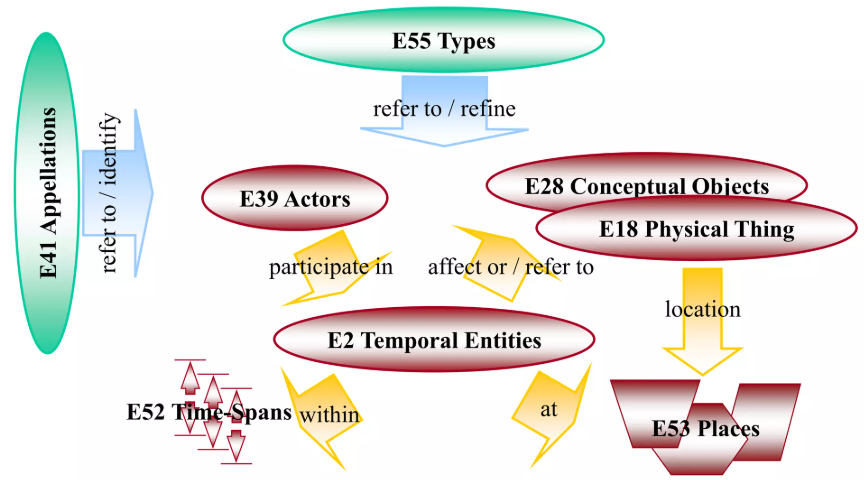
\includegraphics[width=0.7\linewidth]{CIDOC_ISO21127}
    \caption{Fundamental concepts of \texttt{ISO 21127}~\cite{doerr2007cidoc}}.
    \label{fig:cidoc}
\end{figure}
\FloatBarrier

\newpage

\noindent \textbf{From database to \gls{CIDOC-CRM}} \\
The necessary information is extracted from different archaeological and museum collection data models (with various structured, as well as non-structured
data, i.e. text description) to a common standard based on \gls{CIDOC-CRM} compliant structure.
Although the \gls{CIDOC-CRM} model provides a common, standardized framework for representing data from archaeological and museum collections, it has limitations in representing the characteristics of digital \gls{3D} artefacts.



\section{Cultural Heritage Cloud}
\label{sec:ch_cloud}

The \gls{ECCCH}\footnote{\label{myfootnote}https://www.echoes-eccch.eu/}   is a European Union initiative 
to create a shared digital infrastructure that connects \gls{CH} institutions and professionals across the \gls{EU}.
The \gls{ECCCH} aims to add a digital dimension to \gls{CH} preservation, conservation, restoration, and enhancement 
by providing cutting-edge technology for artefact digitisation and artwork research. 
In Portugal, the \gls{ICOM}\footnote{\url{https://icom-portugal.org/}} is a beneficiary of the initiative, while \gls{CRUSOE}\footnote{\url{https://redcrusoe.com/}} is an \gls{ECCCH} association partner. \gls{CRUSOE} is a university association comprising institutions from both Portugal and Spain.
While \gls{ICOM} Portugal and \gls{CRUSOE} represent the participants in Portugal, the \gls{ECCCH} also includes other 14 countries' beneficiaries, affiliated entities and/or associated partners across Europe that actively support those \gls{CH} sectors enumerated above.


\begin{figure}[h!]
    \centering
    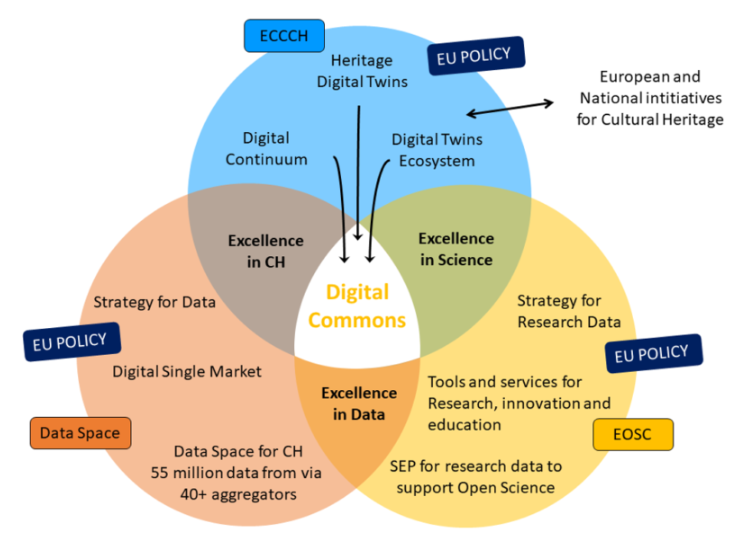
\includegraphics[width=0.7\linewidth]{echoes}
    \caption{\gls{ECHOES} goals \ref{myfootnote}.} 
    \label{fig:echoes}
\end{figure}
\FloatBarrier

